\question 设栈S和队列Q的初始状态均为空,元素a,b,c,d,e,f,g依次进入栈S。若每个元素出栈后立即进入队列Q,且7个元素出队的顺序是b,d,c,f,e,a,g,则栈S的容量至少是(
~)
\par\twoch{1}{2}{\textcolor{red}{3}}{4}
\begin{solution}首先队列不改变进出序列,故本题等价于入栈顺序a,b,c,d,e,f,g。出栈顺序为b,d,c,f,e,a,g,求栈空间至少多大。栈操作的过程如下所示,可以看到,栈中最多有3个元素,即栈大小至少为3。
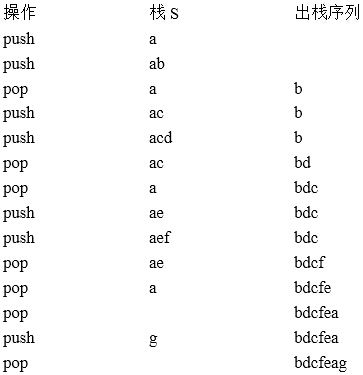
\includegraphics[width=3.78125in,height=3.90625in]{computerassets/13bba34f34f8765d413e9d53bfddf745.jpeg}
【总结】
栈和队列相关的题目并不难,只要根据入栈顺序和出栈顺序,还原栈操作过程,就能够得到正确的答案。
\end{solution}
\question (武汉大学,2005年)设栈S和队列Q的初始状态为空,6个元素入栈的顺序为:a1,a2,a3,a4,a5,a6。一个元素出栈后立即进入队列Q,若6个元素出队的顺序是:a2,a4,a3,a6,a5,a1,则栈S的容量至少应该是(
)
\par\twoch{2}{\textcolor{red}{3}}{4}{6}
\begin{solution}考察栈和队列的特点。栈的特点是后进先出,而队列是先进先出,当a2出栈时,栈中还有a1,当a4出栈时,栈中有元素a1,a3,即此时栈的容量至少为3,当a6出栈时,栈中还有元素a5和a1,故栈S的容量至少为3
\end{solution}
\question 输入受限的双端队列是指元素只能从队列的一端输入,但可以从队列的两端输出,如图所示。若有8、1、4、2依次进入输入受限的双端队列,则得不到输出序列(
~)。~

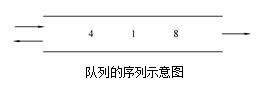
\includegraphics[width=2.75000in,height=0.97917in]{computerassets/95a34a22ed1cd42d10a23b488d7f98e8.png}
\par\fourch{2、8、1、4}{1、4、8、2}{4、2、1、8}{\textcolor{red}{2、1、4、8}}
\begin{solution}A选项:首先,8、1、4、2都从左端入队,然后2从左端出队,8从右端出队,1从右端出队,4从左端出队,得到A的序列。
B选项:首先,8和1分别从左端输入,然后1从左端出队,4再从左端入队,4再从左端出队,2从左端入对,8从右端出队,2从左端出队,得到B的序列。
C选项:首先,8、1、4都从左端入队,4从左端出队,2再从左端入队,2从左端出队,1从左端出队,8从左端或者右端出队,得到C的序列。
D选项:首先,8、1、4、2都从左端入队,然后2从左端出队,队列的序列变成如图所示,接着如果要让1出队列,必须4或8先出队列,所以D的序列不可能实现。

~
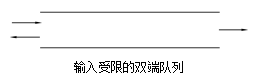
\includegraphics[width=2.67708in,height=0.85417in]{computerassets/5165378b619f5b040e98b8bafb986fda.png}
\end{solution}
